
\documentclass{article}
\usepackage[utf8]{inputenc}
\usepackage[english]{babel}

\usepackage{graphicx}
\usepackage[a4paper, total={6.5in, 10in}]{geometry}
\graphicspath{{./images/}}
\usepackage{wrapfig}
\usepackage{lipsum}
\usepackage{multicol}
\setlength{\columnsep}{20pt}
\usepackage{hyperref}
\usepackage{enumitem}
\usepackage[utf8]{inputenc}
\usepackage[english]{babel}

\setlength{\parskip}{0.3em}
% \usepackage[document]{ragged2e}

\raggedbottom
\raggedcolumns



\title{Machine Learning Algorithms for Fake or Real News Detection}

\author{Ziqian Xu, Yinuo Hu, Mingli Zhang, Xinran Ming}
\date{}

\begin{document}
\maketitle


\begin{multicols}{2}
\section{Introduction}

Fake news are gaining attention nowadays both due to the increasing use of internet and medias and due to the rise in political, social, and cultural awareness. News sources such as \emph{The Onion} which intentionally publish fake information are also attracting attentions (Brodie, 2018). Thus, it has become more and more important for people to be able to identify the truthfulness of news and associated information.\par

Previous studies have attempted to use machine learning algorithms to distinguish fake news from real ones. Researchers have used Logistic Regressions, Naive Bayes algorithms, Support Vector Machines, and Decision Trees to classify news (Katsaros et al., 2019; Granik et al., 2017). Different types of artificial neural networks including Long Short-Term Memory (LSTM) Recurrent Neural Networks, Convolutional Neural Networks, and Adversarial Neural Networks were also widely used in fake information detection tasks (Bahad et al., 2019; Wang et al., 2018; Yang et al., 2018). \par

Because of the plethora of algorithms available to classify fake and real news, and because of the abundance of information with different qualities which are present in our lives, there is a need to explore the effectiveness of different machine learning methods on news classification. Taken together, in the current project, we aim to compare the accuracies of Logistic Regression, Naive Bayes, Support Vector Machine, and LSTM neural network in classifying fake and real news. 


\section{Data and Preprocessing}

\subsection{Data}
We obtained two datasets, one with all fake news (N = 23481) and one with all real news (N = 21417), from https://www.kaggle.com/clmentbisaillon/fake-and-real-news-dataset. The datasets each contains 4 columns representing the title of the news, the text content of the news, the subject of the news, and the date for which the news are posted. 

We used python with a variety of libraries in this project. We used pandas, numpy, matplotlib, seaborn, nltk, and wordcloud for simple text data manipulations and visualizations; we used scikit-learn and keras for modeling.

\subsection{Preprocessing}

\subsubsection{Merging Data}
We first added an additional indicator variable indicating fake (1) or real (0) in the both the real news dataset and the fake news dataset. Then, we merged the two datasets into a complete dataset containing all the news (N = 44898). 

\subsubsection{Text Cleaning}
We used the text contents of the news to classify whether they are real or fake. To do so, we first conducted the following steps to clean up text content of each news article:


\begin{itemize}[noitemsep]
  \item remove text sections that are the news article tagging someone (e.g. "@aPerson").
  \item remove urls in the news articles (e.g. "https://twitter.com/").
  \item remove text sections that are not exactly urls but also contain slash (e.g. "pic.twitter.com/wiQSQNNzw0").
  \item remove "(Rueter)" and anything that comes before it. Real news in the datasets being used often begin with a location for the news and "Rueter" to indicate realness (e.g. "WASHINGTON(Rueter)...").
  \item remove punctuation.
  \item remove numbers and non-alphabetic characters.
  \item remove stop words, which are common words in a language that do not have specific semantic or syntactic significance (e.g. "the", "is").
  \item stem words into root forms to avoid different forms of the same word being treated as separated words (e.g. "drink" and "drinking" should be treated in the same way).
\end{itemize}

For example, the following sentence from real news "WASHINGTON (Reuters) - The U.S. House of Representatives on Thursday approved an \$81 billion bill to help widespread recovery efforts from hurricanes and wildfires this year." became "the us hous repres thursday approv billion bill help widespread recoveri effort hurrican wildfir year" after text cleaning.

\section{Exploratory Data Analysis}


\begin{center}
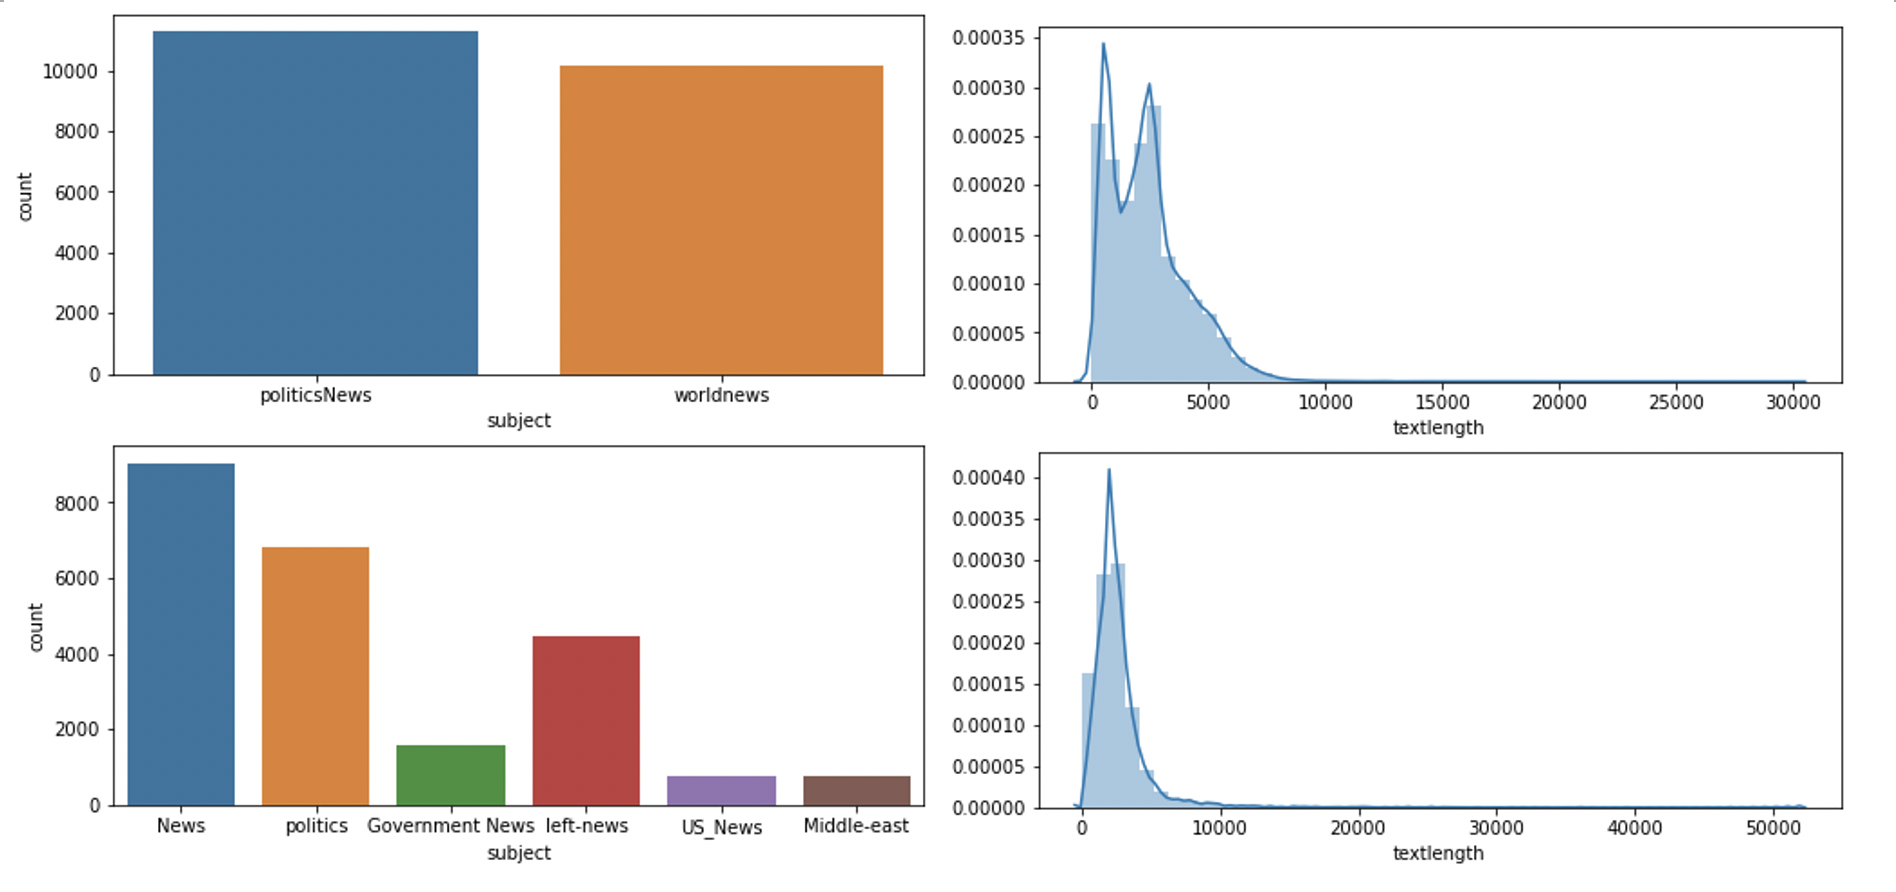
\includegraphics[scale=0.25]{images/img4.png}
\end{center}

We explored the distributions of key news text features as preliminary analyses prior to building machine learning models. While real news only contained subjects of politics or world news, fake news included six categories of subjects, including: news, politics, government news, left-news, US news, and Middle East news. The distributions are shown in the figure above. Real and fake news also had different distributions of text length as shown in the figure above: while real news had two peak lengths with most articles, fake news only had one of such peak, so, text length may be a good indicator of whether a news article is fake or real.  


\begin{center}
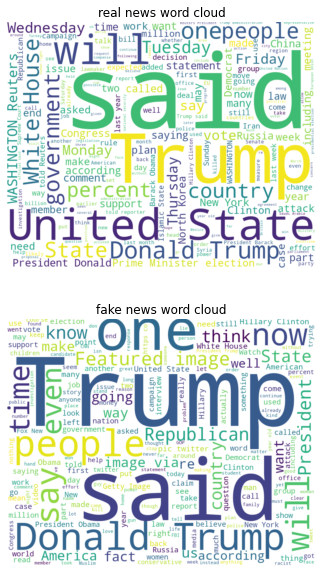
\includegraphics[scale=0.45]{images/wd2.png}
\end{center}

We also looked at the text composition of real versus fake news. The above word cloud figures show which words appear most frequently in the real news dataset and in the fake news dataset respectively. For both real news and fake news, a lot of them are related to the president of U.S. and are about politics. The difference in word composition between real and fake news are not clear from visual inspections of the word clouds, which is why we need to build machine learning models to classify them. The following bar charts show real (top figure) and fake (bottom figure) news word frequency distributions concordant to the top 50 most frequent words extracted by the word clouds shown above. The word frequency distributions used raw data instead of the cleaned up data because whole words make more sense than stemmed words.

\begin{center}
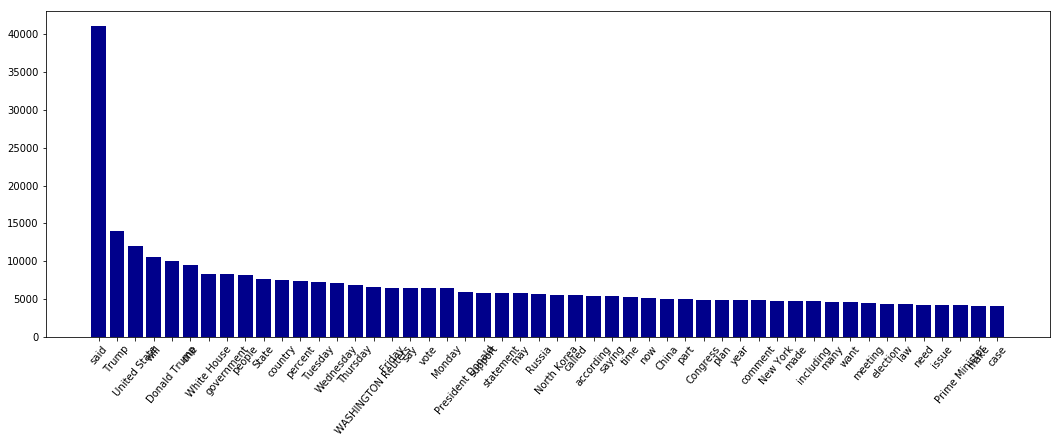
\includegraphics[scale=0.26]{images/freqreal.png}
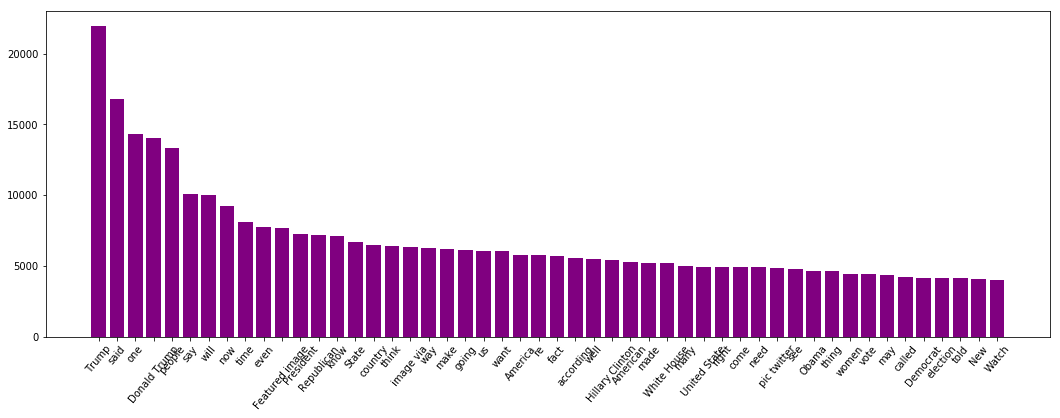
\includegraphics[scale=0.26]{images/freqfake.png}
\end{center}

\section{Models}
\subsection{Text Encoding}
We used different encoding methods for different models. 
For Logistic Regression, Naive Bayes, and Support Vector Machine, we used term frequency–inverse document frequency (TFIDF) to encode news text data into a sparse real-number matrix. For LSTM neural networks, we tokenized the news text corpus and used integer-encoding of each word as representation of data.

\subsection{Training and Testing}
To split training and testing set, we first drop columns with empty news article text. We then randomly chose 90\% of data to be the training set (N = 39764) and the rest 10\% of data to be the testing set (N = 4419).

\subsection{Logistic Regression}
Logistic Regression is widely used for binary classification problems. Logistic Regression uses the sigmoid function, $sigmoid(z)=  \frac{1}{1+e^{z}}$, to convert linear relationships into binary cases using $y=\frac{1}{1+e^{-(b+w_1x_1+w_2x_2...)}}$. 

TFIDF transformation gave us 157664 features from the training set news text, and with these features, the Logistic Regression classifier predicts the testing set with an accuracy of 98.05\%.
\begin{center}
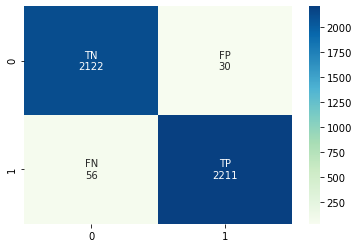
\includegraphics[scale=0.45]{images/lrcm.png}
\end{center}
\subsection{Naive Bayes}
Bayes' Rule states that $P(A|B)=\frac{P(B|A)P(A)}{P(B)}$. Naive Bayes applies Bayes's rule to a chain of features with the assumption that the probability of each feature is independent. There are different types of Naive Bayes classifiers that are based on different distributions such as Bernoulli, Gaussian, and Multinomial. Although the TFIDF encoding we used generates float-point data, Gaussian Naive Bayes classifier cannot be used in our study because it requires a non-sparse input matrix. Thus, we chose to use the Multinomial Native Bayes classifier, which would work with TDIDF data even though discrete encoding would be more ideal. 

After training with 157664 features, the Multinomial Native Bayes classifier predicts the testing set with an accuracy of 93.32\%.

\begin{center}
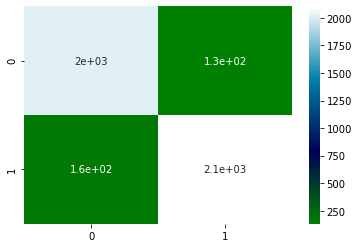
\includegraphics[scale=0.45]{images/nbcm.png}
\end{center}

\subsection{Support Vector Machine}
Support Vector Machine (SVM) is another supervised machine learning algorithm often used for classification tasks. Unlike Logistic Regression, SVM uses the orthogonal distances from the decision boundary that separates different labels to the data points near the boundary to decided how to optimize the classification task. 

After training with 157664 features, the SVM classifier predicts the testing set with an accuracy of 98.23\%.

\begin{center}
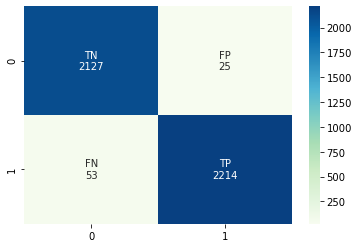
\includegraphics[scale=0.45]{images/svmcm.png}
\end{center}

\subsection{LSTM}
We also used a bi-directional LSTM recurrent neural network suggested by Bahad et al. (2019) for text classification of real versus fake news. Bi-directional LSTM is a form of generative learning algorithm that connects hidden layers of two opposite directions as an attempt to connect what comes later with what comes before (Schuster \& Paliwal, 1997). This is particularly useful in natural language processing such as text classification tasks because what comes later in a sentence may need to be combined with what comes earlier in a sentence to make sense.

\begin{center}
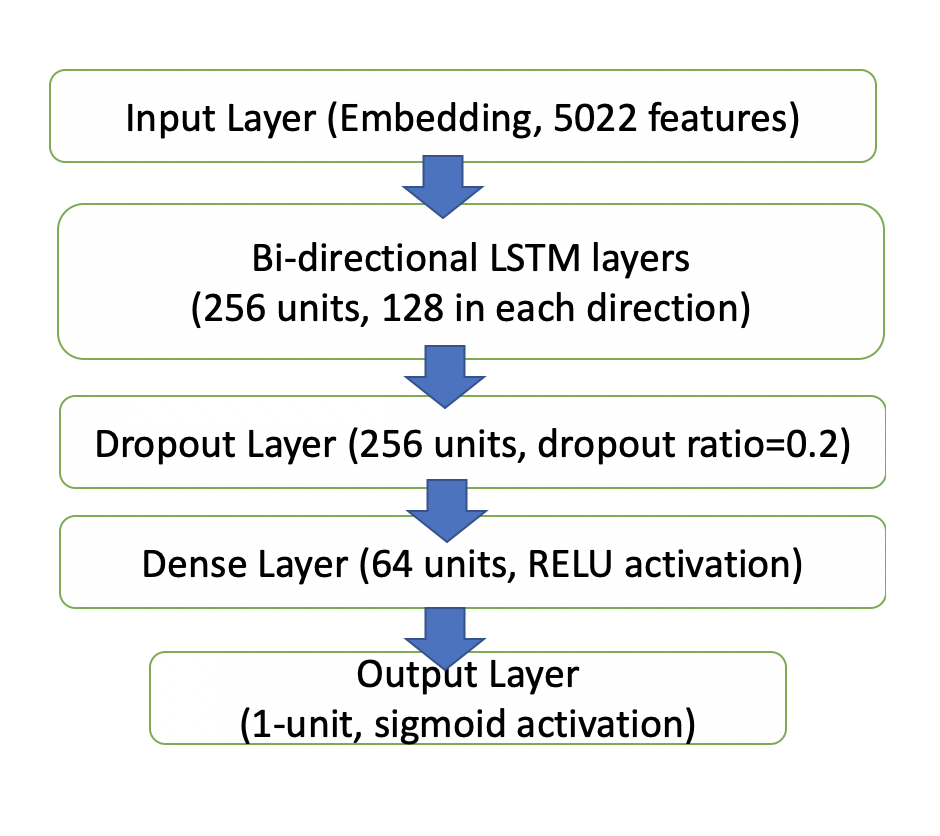
\includegraphics[scale=0.35]{images/img5.png}
\end{center}

We used the above network structure with one iteration of the bi-directional LSTM layes followed by a dropout layer to prevent over-fitting. Two dense layers are used after the LSTM layers to generate the desired output. We trained this network with 5022 features in 39764 training samples over 5 epochs with a mini-batch size of 128.


This bi-directional LSTM neural network predicts the testing dataset with an accuracy of 98.73\%.

\begin{center}
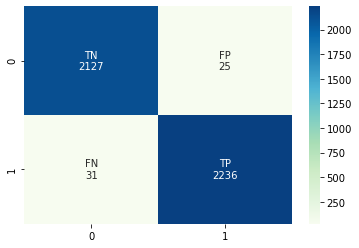
\includegraphics[scale=0.45]{images/lstmcm.png}
\end{center}

\section{Conclusions}

\subsection{Model Comparison}


Comparing the models above, the Naive Bayes classifier has the lowest accuracy while the LSTM network has the highest accuracy. However, although Naive Bayes has the lowest accuracy, the score is still above 90\%. On the other side, while LSTM has the highest score, LSTM's accuracy is only marginally better than Logistic Regression and SVM. This being said, running more epochs during the training phase of LSTM may further increase the score. Admittedly though, LSTM is significantly more computational expensive than the other algorithms, so the decision of which model to use may depend on both what accuracy level is needed and what computational power and time requirements are present. 

Another thing to note is that although LSTM's accuracy is only slightly higher than the other machine learning models used in this project, we did train the LSTM model using much fewer features. The Logistic Regression, Support Vector Machine, and Naive Bayes had 157664 features to train on whereas for the LSTM model, we only used 5022 features for training.

The following table shows the accuracies, true negatives (TNs), true positives (TPs), false negatives (FPs), and false positives (FPs) of the algorithms used in this study for classifying real vesus fake news. 


\begin{center}
\begin{tabular}{ c| c c c c c}
 model & accuracy & TN & TP & FN & FP \\ 
\hline
LR & 98.05\% & 2122  & 2211 & 56 & 30\\ 
NB & 93.32\% & 2020 & 2104 & 163 & 132\\
SVM & 98.23\% & 2127 & 2214 & 53 & 25\\
LSTM & 98.73\% & 2127 & 2236 & 31 & 25 \\
\end{tabular}
\end{center}

\subsection{Future Directions}

Machine learning algorithms are relatively accurate in predicting fake news from the news articles' text content. However, because news articles can be long, processing and categorizing article texts maybe inefficient in computation and training time. In the future, we may want to investigate whether instead of news article contents, news title lines can be used to predict news articles' truthfulness. News title lines are much shorter than the actual contents of news articles, thus can be more computationally efficient to analyze. 




\section{Acknowledgements}

We thank the following kaggle kernels for guiding us through the natural language processing tasks:
\begin{itemize}
    \item https://www.kaggle.com/parulpandey/getting-started-with-nlp-a-general-intro
    \item https://www.kaggle.com/nasirkhalid24 /unsupervised-k-means-clustering-fake-news-87
    \item https://www.kaggle.com/muhammadshahzad
    khan/is-it-real-news-nlp-lstm-acc-99-9#Now-we-need-to-apply-padding-to-make-sure-that-all-the-sequences-have-same-length
\end{itemize}


\section{References}

\quad \, Ahmed, H., Traore, I., \& Saad, S. (2018). Detecting opinion spams and fake news using text classification. Security and Privacy, 1(1), e9.

Bahad, P., Saxena, P., \& Kamal, R. (2019). Fake News Detection using Bi-directional LSTM-Recurrent Neural Network. Procedia Computer Science, 165, 74-82.

Brodie, I. (2018). Pretend news, false news, fake news: The onion as put-on, prank, and legend. Journal of American Folklore, 131(522), 451-459.

Granik, M., \& Mesyura, V. (2017, May). Fake news detection using naive Bayes classifier. In 2017 IEEE First Ukraine Conference on Electrical and Computer Engineering (UKRCON) (pp. 900-903). IEEE.

Katsaros, D., Stavropoulos, G., \& Papakostas, D. (2019, October). Which machine learning paradigm for fake news detection?. In 2019 IEEE/WIC/ACM International Conference on Web Intelligence (WI) (pp. 383-387). IEEE.

Schuster, M., \& Paliwal, K. K. (1997). Bidirectional recurrent neural networks. IEEE transactions on Signal Processing, 45(11), 2673-2681.

Wang, Y., Ma, F., Jin, Z., Yuan, Y., Xun, G., Jha, K., ... \& Gao, J. (2018, July). Eann: Event adversarial neural networks for multi-modal fake news detection. In Proceedings of the 24th acm sigkdd international conference on knowledge discovery & data mining (pp. 849-857).

Yang, Y., Zheng, L., Zhang, J., Cui, Q., Li, Z., \& Yu, P. S. (2018). TI-CNN: Convolutional neural networks for fake news detection. arXiv preprint arXiv:1806.00749.

\end{multicols}
\end{document}


